\documentclass{article}
\usepackage[T1]{fontenc}
\usepackage[utf8]{inputenc}
\usepackage{listings}
\usepackage{color}
\definecolor{red}{rgb}{0.6,0,0} % for strings
\definecolor{green}{rgb}{0.25,0.5,0.35} % comments
\definecolor{purple}{rgb}{0.5,0,0.35} % keywords
\definecolor{docblue}{rgb}{0.25,0.35,0.75} % javadoc
 
\lstset{
	basicstyle=\normalsize\ttfamily,
	keywordstyle=\color{purple}\bfseries,
	stringstyle=\color{red},
	commentstyle=\color{green},
	morecomment=[s][\color{docblue}]{/**}{*/},
	tabsize=4,
	showspaces=false,
	showstringspaces=false
}
	
\usepackage{graphicx}
\usepackage{fancyhdr}
\usepackage[margin=1.2in]{geometry}
\geometry{a4paper, left=20mm, right=20mm, top=20mm, bottom=20mm}
\linespread{1.5}
\begin{document}

\begin{titlepage}
	\begin{center}
		{\LARGE College of Engineering, Trivandrum}\\[3cm]
		\linespread{1.2}\huge {\bfseries Microprocessor Lab}\\[3cm]
		\linespread{1}
		
\includegraphics[width=8cm]{img/emblem.jpeg}\\[1cm]
		{\Large Gokul K\\ S6 CSE \\ Roll No: 21\\ TVE18CS021 }\\[1cm]
		\textit{ }\\[1cm]
		{\LARGE 
			Department of Computer Science\\[0.2cm]
			\today 
		}
	\end{center}
	
\end{titlepage}
\large

\newpage
\setlength{\headheight}{15.2pt}
\pagestyle{fancy}
\fancyhf{}
\fancyhead[RO]{\fontsize{12}{12}\selectfont\nouppercase\leftmark} 
\fancyhead[LO]{\fontsize{9}{12}\selectfont\nouppercase\rightmark} 

\setcounter{section}{7}

% Use the current experiment file from experiments/ folder
\section{Fibonacci sequence}
\subsection{Aim}
To generate first n Fibonacci numbers.

\subsection{Code}
\begin{lstlisting}
ORG 0000H

MOV R0, #08H
MOV DPTR, #100H

MOV A, #00H
MOVX @DPTR, A
INC DPTR
MOV A, #01H
MOVX @DPTR, A

LOOP:
	MOV A, DPL
	SUBB A, #1
	MOV DPL, A
	MOV A, DPH
	SUBB A, #0H
	MOV DPH, A

	MOVX A, @DPTR
	INC DPTR
	MOV R1, A
	MOVX A, @DPTR
	INC DPTR
	ADD A, R1
	MOVX @DPTR, A

	DJNZ R0, LOOP
END
\end{lstlisting}

\subsection{Output}
\textbf{Input} 08H (R0)\\
\textbf{Output} 00H, 01H, 01H, 02H, 03H, 05H, 08H, 0DH, 15H, 22H (At locations from \#100H of XDATA)\\
\begin{center}
	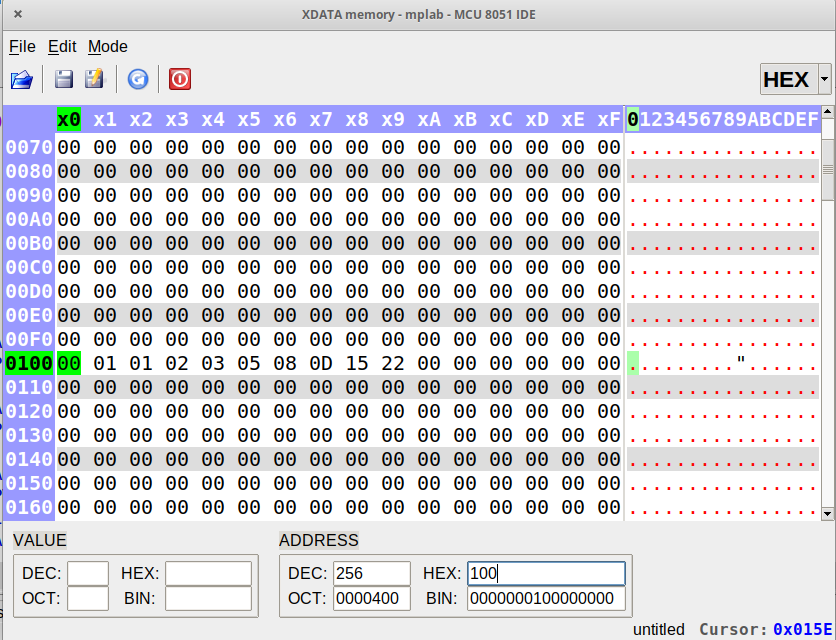
\includegraphics[width=\textwidth]{img/p28.png}
\end{center}


\subsection{Result}
First n Fibonacci sequence was generated in mcu8051ide

\newpage
\section{Largest and smallest of an array}
\subsection{Aim}
To find the largest and smallest of 8-bit numbers

\subsection{Code}
\begin{lstlisting}
ORG 0000H

MOV DPTR, #100H
MOV R0, #08H
MOV R1, #7FH
MOV R2, #00H

LOOP:
	MOVX A, @DPTR
	SUBB A, R2
	JNC LARGE
CHECKSMALL:
	MOVX A, @DPTR
	SUBB A, R1
	JC SMALL
	JNC INCREMENT
	
LARGE:
	MOVX A, @DPTR
	MOV R2, A
	JMP CHECKSMALL

SMALL:
	MOVX A, @DPTR
	MOV R1, A

INCREMENT:
	INC DPTR
	DJNZ R0, LOOP
	
END
\end{lstlisting}

\subsection{Output}
\textbf{Input} 18H, 17H, 16H, 15H, 20H, 21H, 21H, 18H (at locations starting from \#100H on XDATA)\\
\textbf{Output} 15H (R1) (Smallest of the array) and 21H (R2) (Largest of the array)\\
\begin{center}
	\includegraphics[width=\textwidth]{img/p29/ss1.png}
\end{center}
\begin{center}
	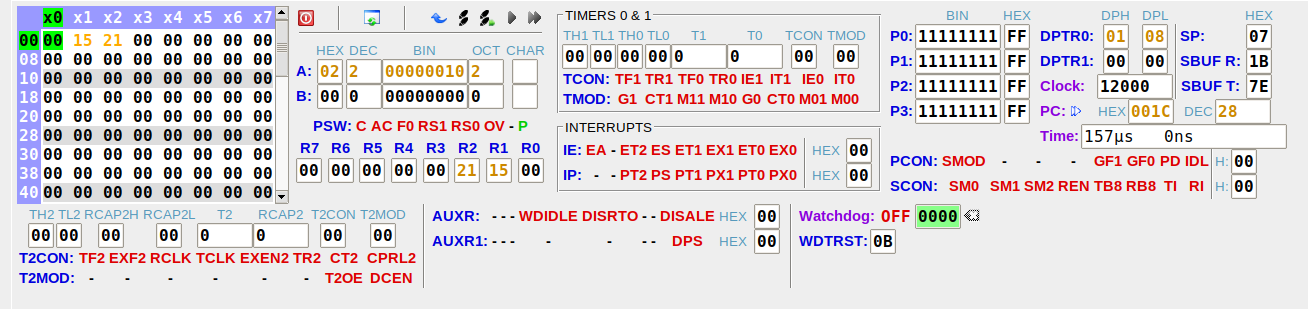
\includegraphics[width=\textwidth]{img/p29/ss2.png}
\end{center}


\subsection{Result}
Largest and smallest elements of an array was found on mcu8051ide

\newpage
\section{Bubble sort}
\subsection{Aim}
To perform bubble sort on 8-bit numbers

\subsection{Code}
\begin{lstlisting}
ORG 0000H

startaddr EQU 100H

MOV R0, #08H
MOV R1, #00H

MOV DPTR, #startaddr

DEC R0
MOV A, R0
MOV R1, A

OUTERLOOP:
	MOV A, R0
	MOV R2, A
	MOV DPTR, #startaddr
INNERLOOP:
	MOVX A, @DPTR
	MOV R3, A
	INC DPTR
	MOVX A, @DPTR
	SUBB A, R3
	JNC INNERLOOP_INCR

	MOVX A, @DPTR
	XCH A, R3
	MOVX @DPTR, A
	DEC DPL
	MOV A, R3
	MOVX @DPTR, A
INNERLOOP_INCR:
	DJNZ R2, INNERLOOP
OUTERLOOP_INCR:
	DJNZ R1, OUTERLOOP

EXIT:
	NOP
END
\end{lstlisting}

\subsection{Output}
\textbf{Input} 18H, 17H, 16H, 15H, 20H, 21H, 21H, 18H (at locations starting from \#100H on XDATA)\\
\textbf{Output} 15H, 16H, 17H, 18H, 18H, 20H, 21H, 21H\\
\begin{center}
	\includegraphics[width=\textwidth]{img/p30/ss1.png}
\end{center}
\begin{center}
	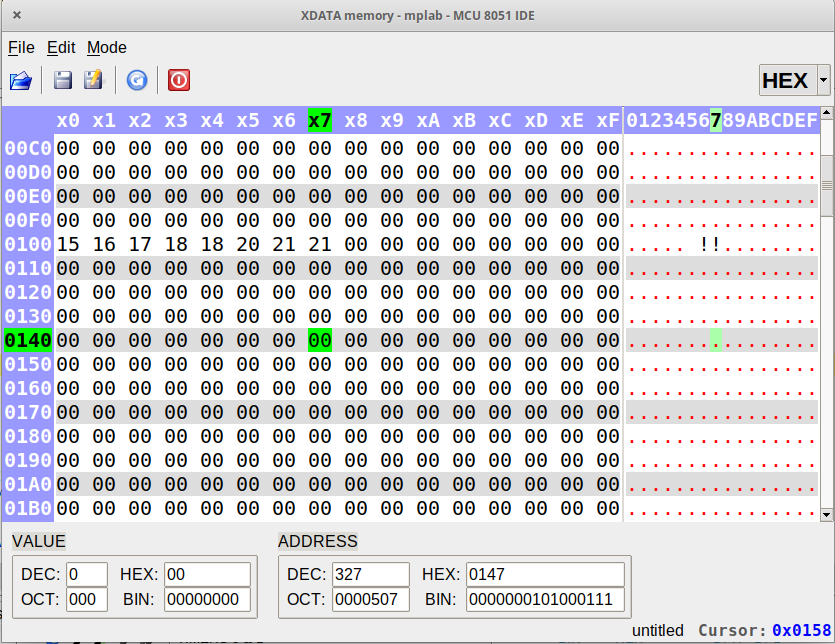
\includegraphics[width=\textwidth]{img/p30/ss2.png}
\end{center}


\subsection{Result}
Bubble sort was performed on an array was found on mcu8051ide

\newpage
\section{Hexadecimal to decimal}
\subsection{Aim}
To implement hex to decimal conversion

\subsection{Code}
\begin{lstlisting}
ORG 0000H

MOV R0, #55H
MOV R1, #00H
MOV R2, #00H

MOV A, R0
MOV B, #100
DIV AB

MOV R0, A
CLR C
MOV A, B
MOV B, #10
DIV AB

SWAP A

MOV R1, A
MOV A, B
ORL A, R1
MOV R1, A

END
\end{lstlisting}

\subsection{Output}
\textbf{Input} 55H (R0))\\
\textbf{Output} 85 (R1)\\
\begin{center}
	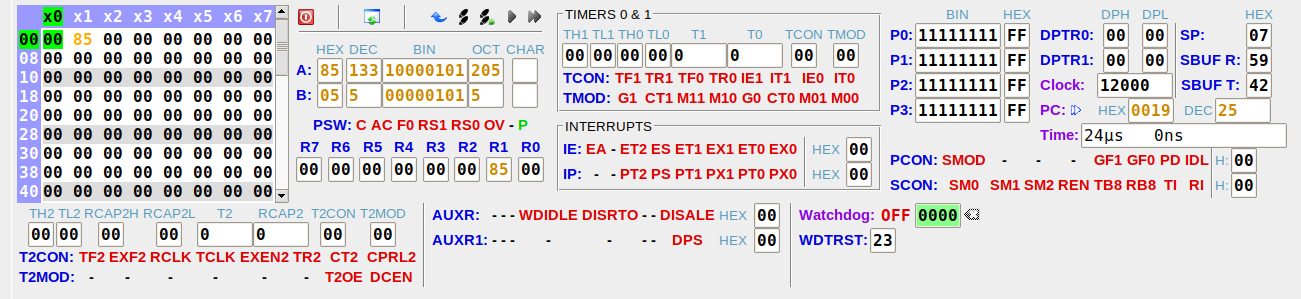
\includegraphics[width=\textwidth]{img/p31.png}
\end{center}


\subsection{Result}
Hexadecimal number was converted to decimal on mcu8051ide

\newpage
\section{Decimal to hexadecimal}
\subsection{Aim}
To implement decimal to hex conversion

\subsection{Code}
\begin{lstlisting}
ORG 0000H

MOV R0, #85H
MOV R1, #00H
MOV A, #00H

LOOP:
	ADD A, #01H
	DA A
	INC R1
	CJNE A, 00H, LOOP ; Run the loop until A = R0

END
\end{lstlisting}

\subsection{Output}
\textbf{Input} 85 (R0))\\
\textbf{Output} 55 (R1)\\
\begin{center}
	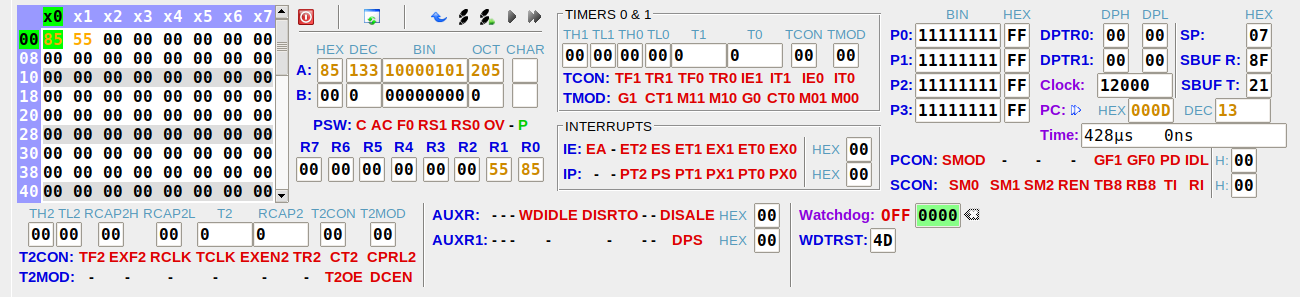
\includegraphics[width=\textwidth]{img/p32.png}
\end{center}


\subsection{Result}
Decimal number was converted to hexadecimal on mcu8051ide
\end{document}